\chapter{Evaluierung} \label{Evaluierung}
Um den Erfolg/Misserfolg, bzw. den praktischen Nutzen dieses Projektes werten und bemessen zu können, wurde eine Evaluierung durchgeführt. Da für die einzelnen Komponenten des Projektes bereits Unit-Tests geschrieben und durchgeführt wurden, und diese in den jeweiligen Kapiteln erläutert sind, befassen wir uns hier ausschließlich mit der Evaluierung des Endproduktes und dessen Anwendung.
\section{Konzept}
Um die Anforderungen aus \textbf{Kapitel X} evaluieren zu können, benötigt es ein Konzept, welches der klinischen Anwendung so nah wie möglich kommt. Zudem müssen Möglichkeiten geschaffen werden, messen zu können inwiefern und wie exakt die Anforderungen erfüllt wurden. Es muss also erstens überprüft werden, ob die Positionen geschallter Objekte mit den projizierten Positionen auf dem Ultraschallbild übereinstimmen. Zudem müssen ebenfalls Distanzen und Größen zwischen realen Objekten und den projizierten Objekten übereinstimmen. Das zu erreichende Ziel ist schließlich, den Effekt zu erzielen, dass die Projektion des Ultraschallbildes eines Objekts das reale Objekt exakt überlagert. 
\\
Um eben aufgezählte Messungen vornehmen zu können benötigte es zunächst ein Testobjekt. Hierbei entschieden wir uns für die Variante einer Gelatineplatte als Phantom, in den zwei Münzen bekannter Größe und Distanz zueinander integriert wurden (siehe Kapitel \ref{Phantom}). 
\clearpage
\section{Versuchsaufbau} \label{Versuchsaufbau}
Für die Herstellung einer dauerhaften Gelatineplatte wie in Kapitel \ref{Phantom} beschrieben, wurden folgende Materielien benötigt:
\begin{itemize}
\item 100ml Wasser
\item 50ml Isopropyl-Alkohol
\item 50ml Glycerin
\item 3,5 Päckchen Gelatine
\item Lebensmittelfarbe
\item Plastikbehälter
\item eine Herdplatte
\item ein Löffel
\item Zeitungspapier o.ä.
\item 2 1-Cent Münzen
\end{itemize}

Zunächst muss man die Gelatine 10min in 100ml kaltem Wasser quellen lassen. Anschließend werden die 50ml Isopropyl-Alkohol und die 50ml Glycerin miteinander vermischt. Ist die Gelatine gequollen, wird das Isopropyl-Alkohol-Glycerin-Gemisch und die Lebensmittelfarbe dazugegeben. Diese Mischung wird nun leicht erwärmt, bis alle Klümpchen sich aufgelöst haben. Nun kann die flüssige Masse in den ausgewählten Plastikbehälter gegossen werden und die Münzen hinzugegeben werden. Luftbläschen, die an die Oberfläche gelangen, werden anschließend mit Zeitungspapier vorsichtig entfernt. Ist die Gelatineplatte fest geworden, kann mit der Evaluierung begonnen werden. Wie in Abbildung \ref{fig:gelatineplatte} zu erkennen ist, beträgt der Durchmesser einer Münze 1,635cm und der Abstand zwischen den beiden Münzen beträgt 2,5cm. Beide Münzen liegen 1,3cm tief in der Gelatine.
\clearpage
\begin{figure}[h]
	\centering
	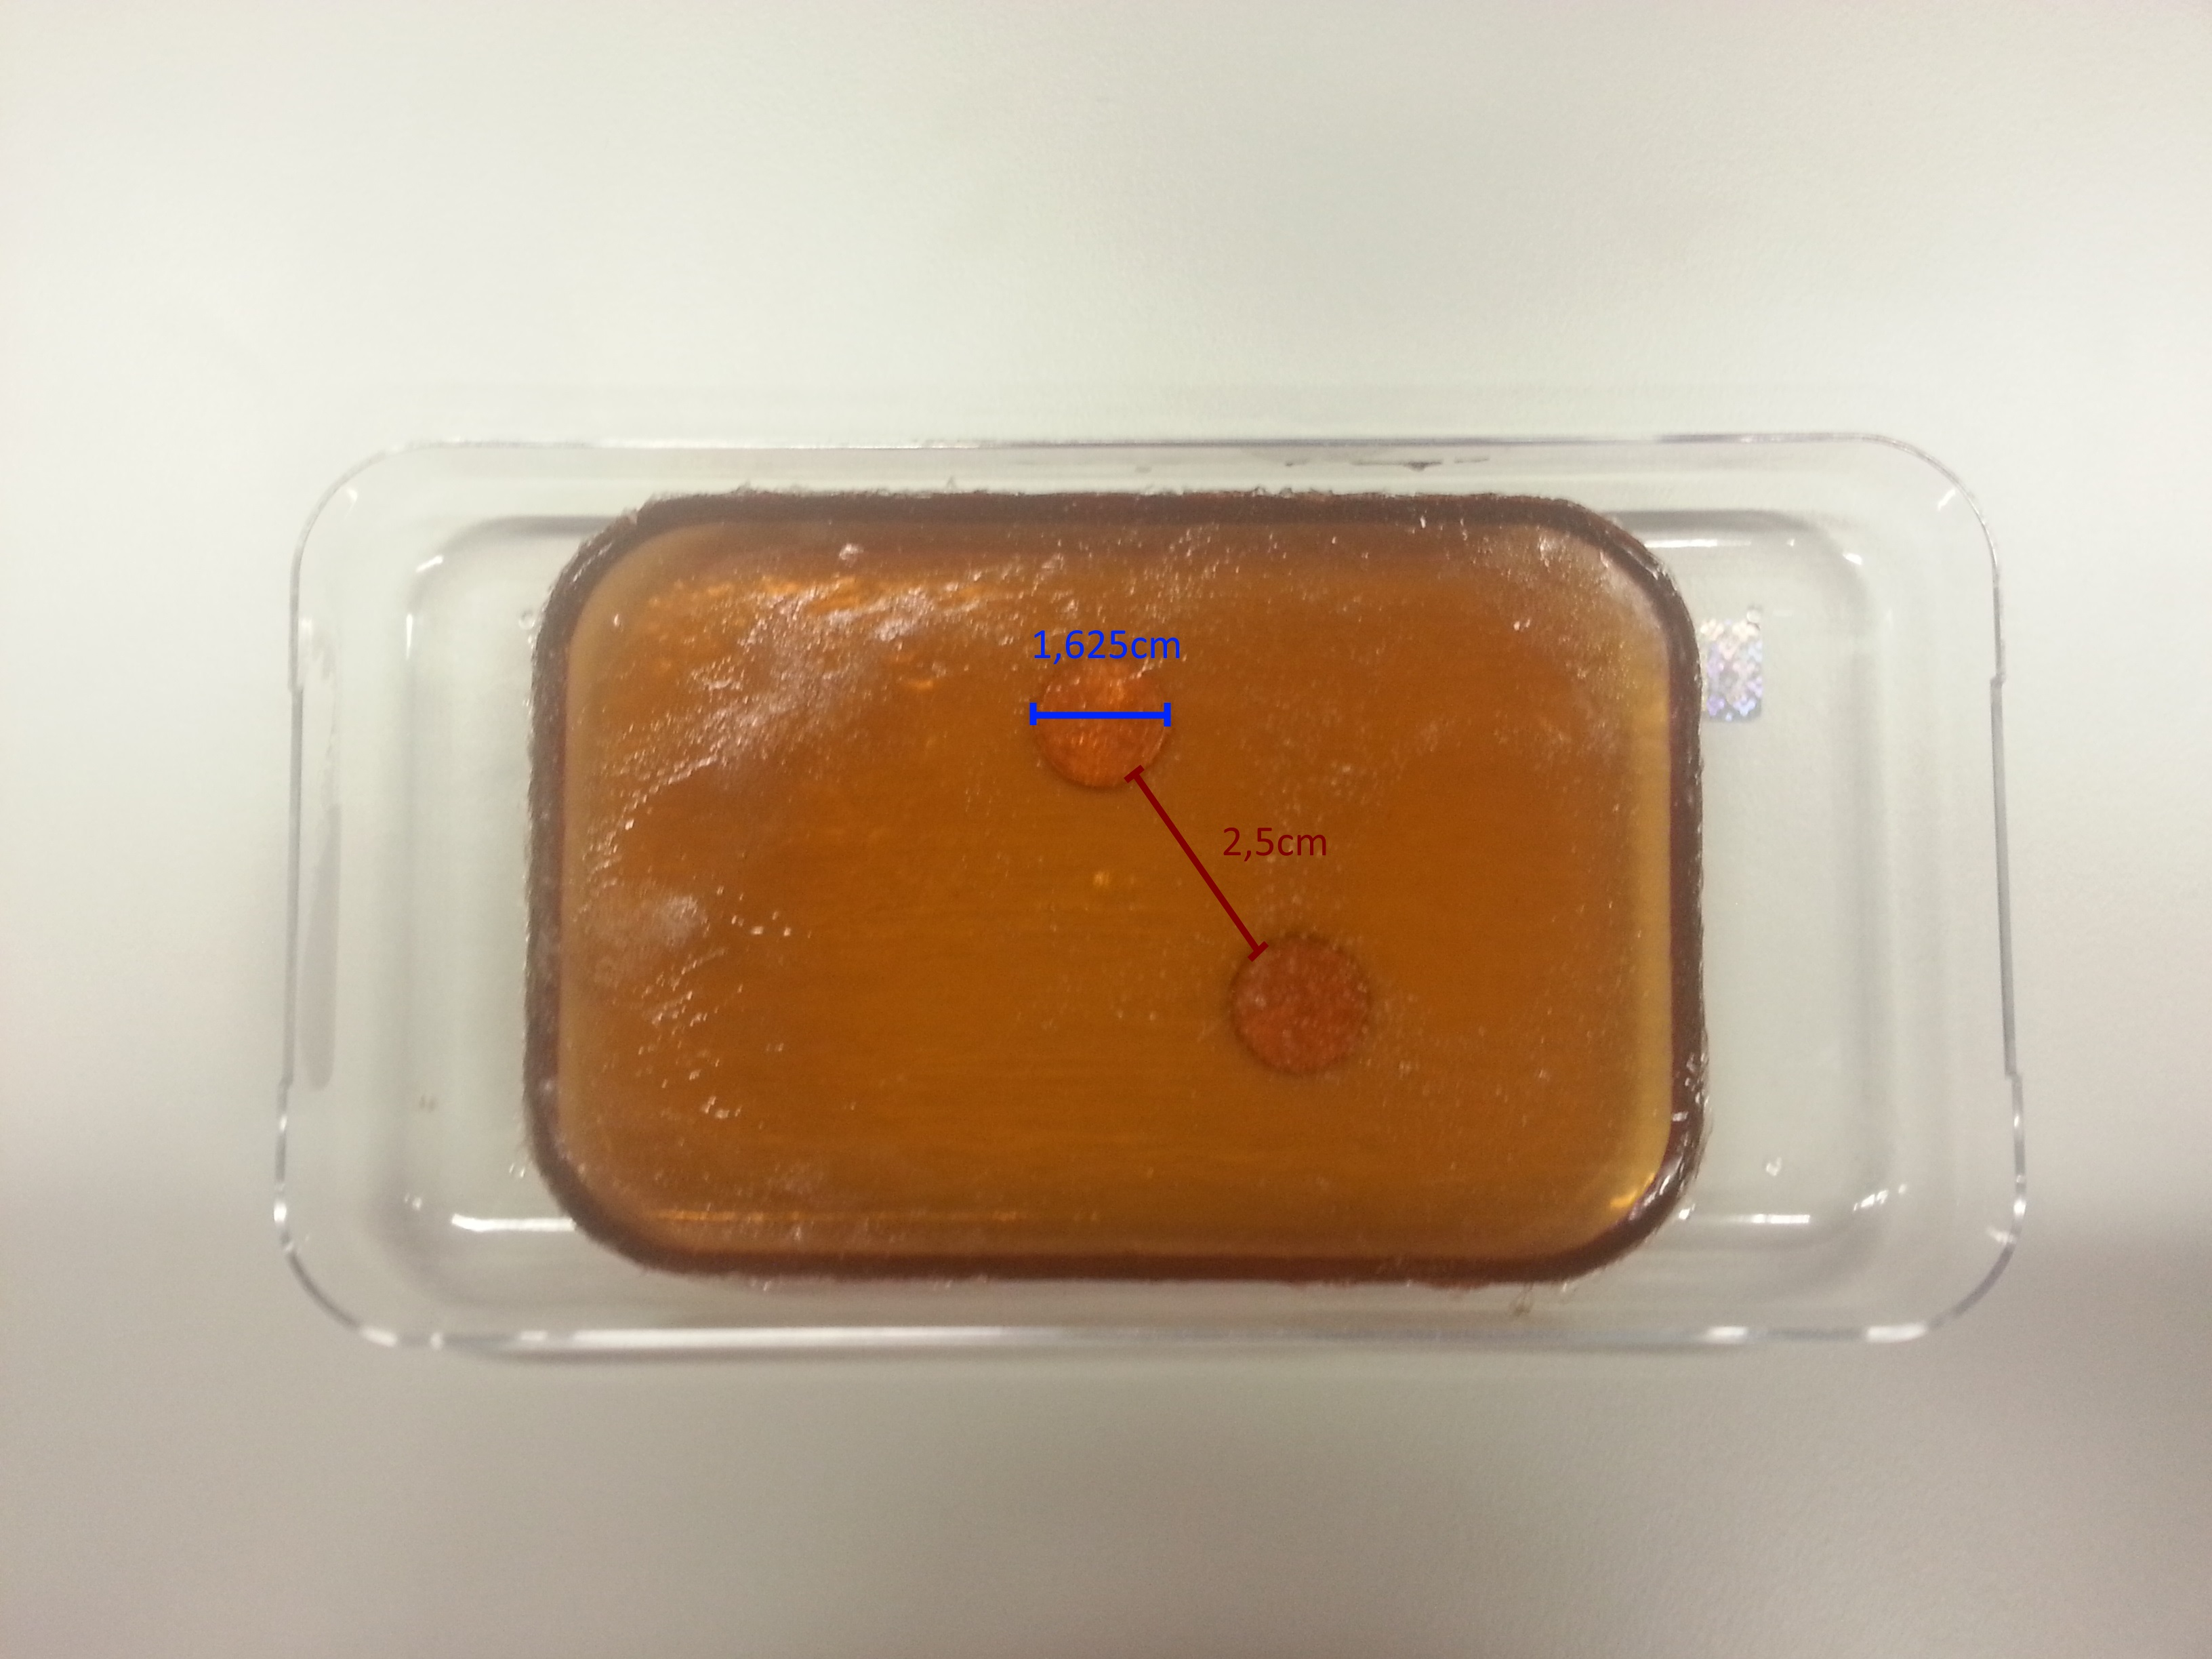
\includegraphics[width=1\textwidth]{Bilder/Evaluation/Gelatineplatte.jpg}
	\caption{Gelatineplatte mit Münzen}
	\label{fig:gelatineplatte}
\end{figure}

\section{Durchführung}
Um Ultraschallbilder der Münzen in der Gelatineplatte aufzunehmen, wird auf diese zunächst Ultraschallgel aufgetragen. Anschließend kann mit dem Prototypen (siehe Kapitel \textbf{X}) das Schallen begonnen werden (siehe Abbildung \ref{fig:schallen}). Geschallt wurde auf zwei Arten: Einmal so, dass der Abstand zwischen den Münzen gut sichtbar auf dem Display zu sehen war und einmal direkt über einer Münze, um ihren Durchmesser auf dem Bild abmessen zu können.
\clearpage
\begin{figure}[h]
	\centering
	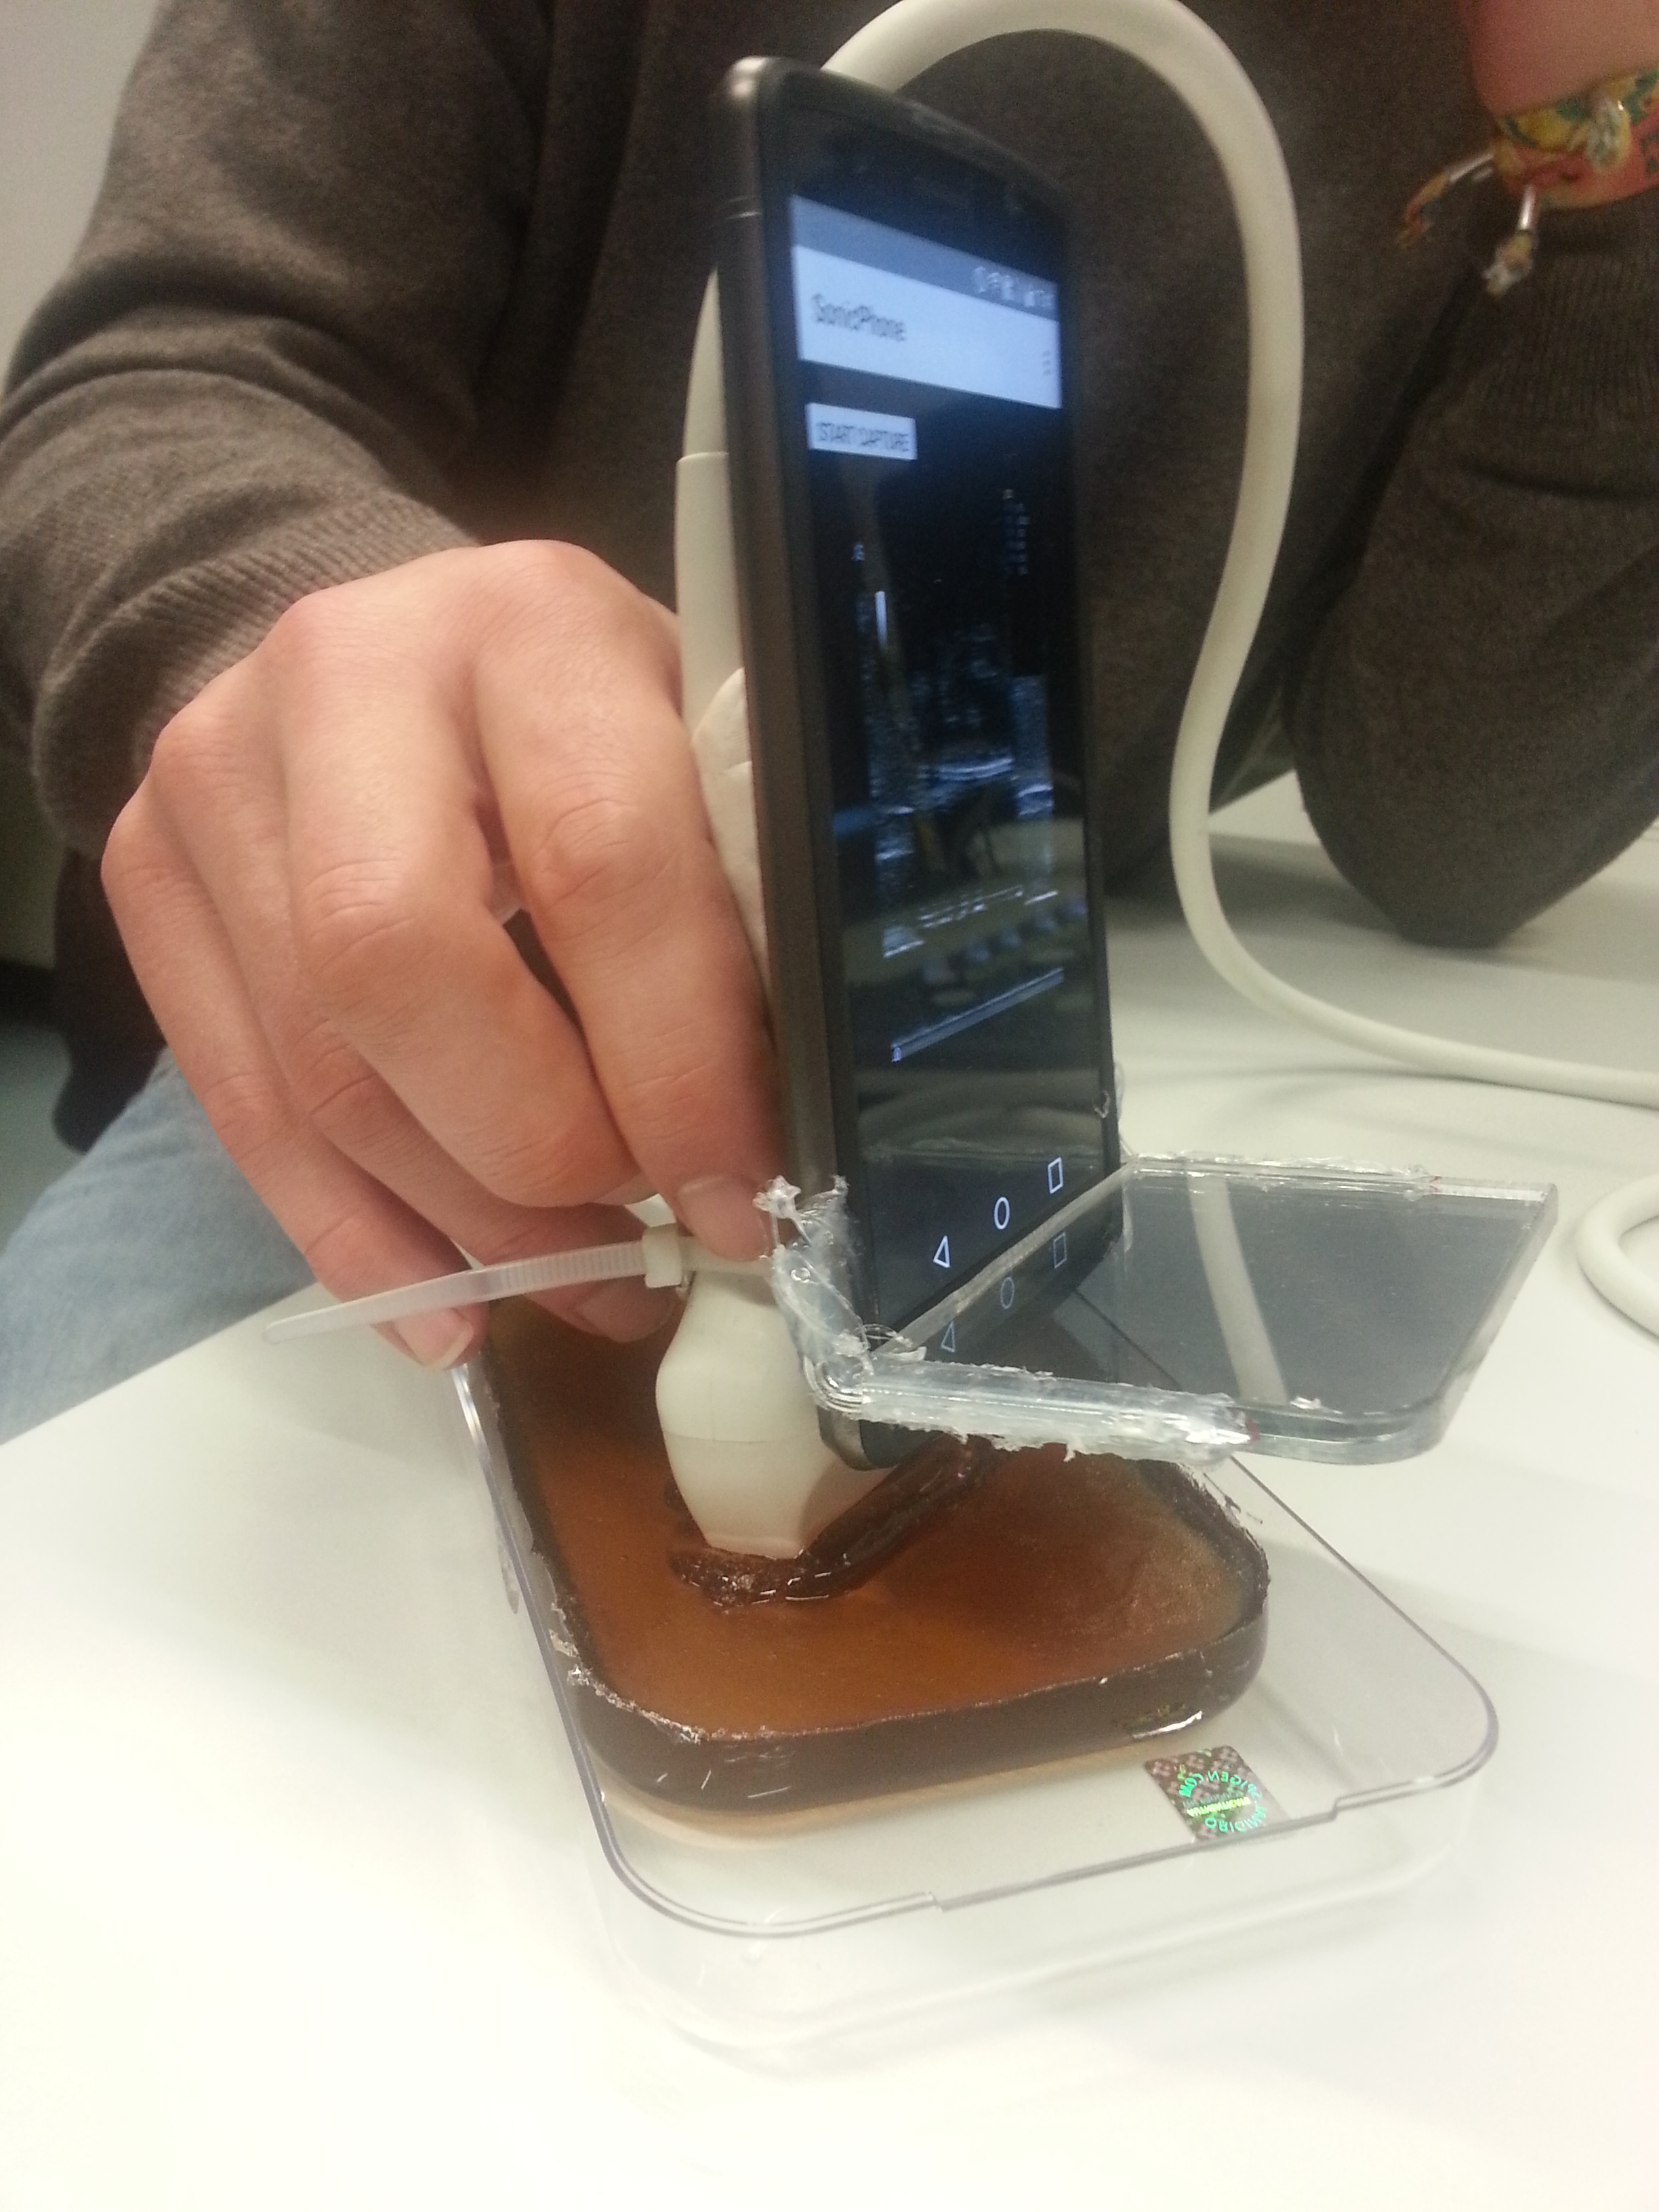
\includegraphics[width=0.6\textwidth]{Bilder/Evaluation/Schallen.jpg}
	\caption{Das Schallen der Gelatineplatte}
	\label{fig:schallen}
\end{figure}

\section{Ergebnisse}
Beim Schallen einer einzelnen Münze konnte die korrekte Tiefe von 1,3cm der Münze in der Gelatineplatte auch im Ultraschallbild abgelesen werden. Der Durchmesser weicht mit gemessenen 1,8cm auf dem Ultraschallbild um 0,175cm vom realen Durchmesser der Münze ab (siehe Abbildung \ref{fig:1Cent}). 
\clearpage
\begin{figure}[h]
	\centering
	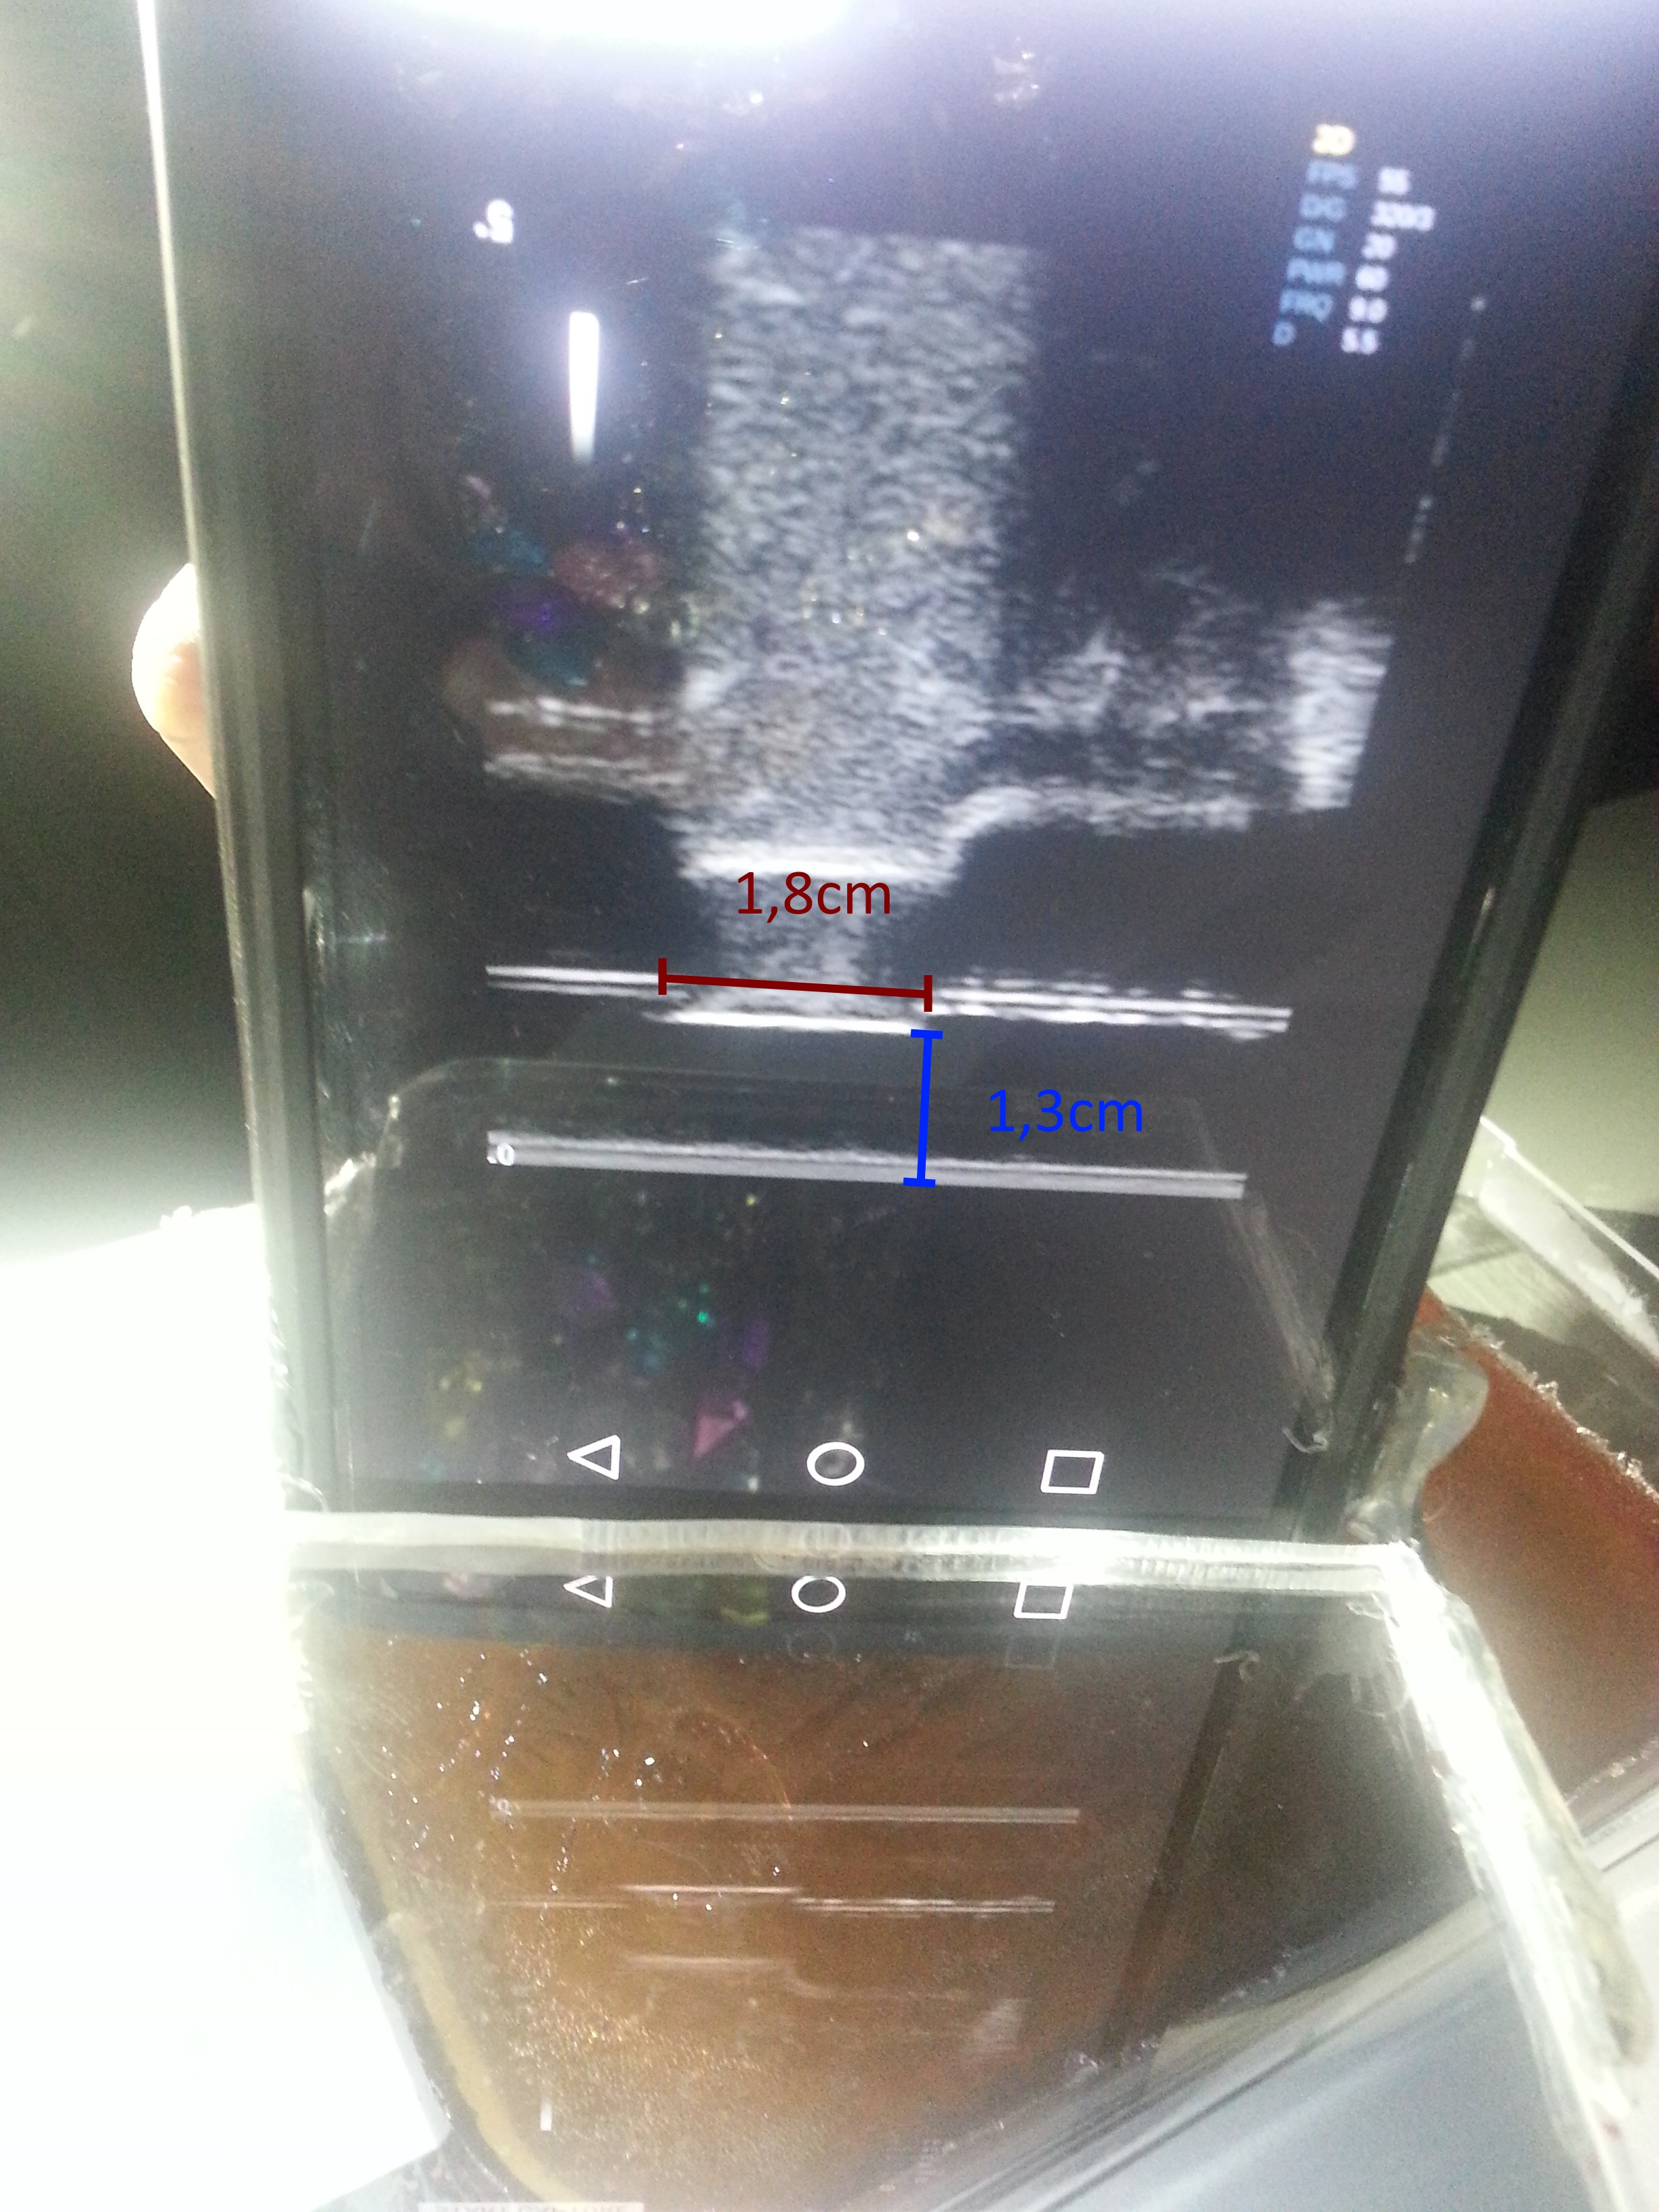
\includegraphics[width=0.5\textwidth]{Bilder/Evaluation/1Cent.jpg}
	\caption{Das Schallen einer Münze in der Gelatineplatte}
	\label{fig:1Cent}
\end{figure}

~\\
Bei diesem ersten Test fiel auf, dass sich die Projektion optisch nicht mit der Münze überlagert. Der Grund hierfür ist, die Distanzen von Ultraschallbild zum Spiegel und Schallkopfende zum Spiegel nicht wie in Kapitel \textbf{X} gefordert und beschrieben übereinstimmten. Der Abstand zwischen Spiegel und Schallkopf beträgt 3,4cm. Der Abstand zwischen Spiegel und Schallbild nur 2,3cm. Um diesen Fehler zu beheben wurde das Ultraschallbild in der Anzeige auf dem Display weiter nach oben verschoben, um die Distanzen \textit{d} zwischen Schallkopf und Spiegel und Schallbild und Spiegel anzugleichen (siehe Abbildung \ref{fig:Prototyp_Evaluierung}). Beide Abstände sind nun identisch und betragen 3,4cm.
\\
Die relevanten Distanzen sind dabei in der Abbildung \ref{fig:Prototyp_Evaluierung} grün dargestellt, das Ultraschallbild auf dem Smartphone-Display violett.
\clearpage
\begin{figure}[h]
	\centering
	\includegraphics*[width=0.7\textwidth]{Bilder/Evaluation/Prototyp.png}
	\caption{Anpassung der Darstellung des Ultraschallbildes auf dem Handy-Display}
	\label{fig:Prototyp_Evaluierung}
\end{figure}

~\\
Nachdem oben beschriebene Anpassungen vorgenommen wurden, wurde ein zweiter Testlauf gestartet. Da die Distanzen nun übereinstimmten, stimmte nun auch die Position der Projektion auf der Gelatineplatte. Dieses Mal wurde der Ultraschallkopf so geführt, dass beide Münzen auf dem Bild zu sehen sind und der Abstand zwischen diesen überprüft werden konnte. Der reale Abstand zwischen den Münzen beträgt, wie in Kapitel \ref{Versuchsaufbau} beschrieben, 2,5cm. Gemessen wurde, wie in Abbildung \textbf{X} zu erkennen ist, ebenfalls ein Abstand von 2,5cm.
\clearpage
\begin{figure}[h]
	\centering
	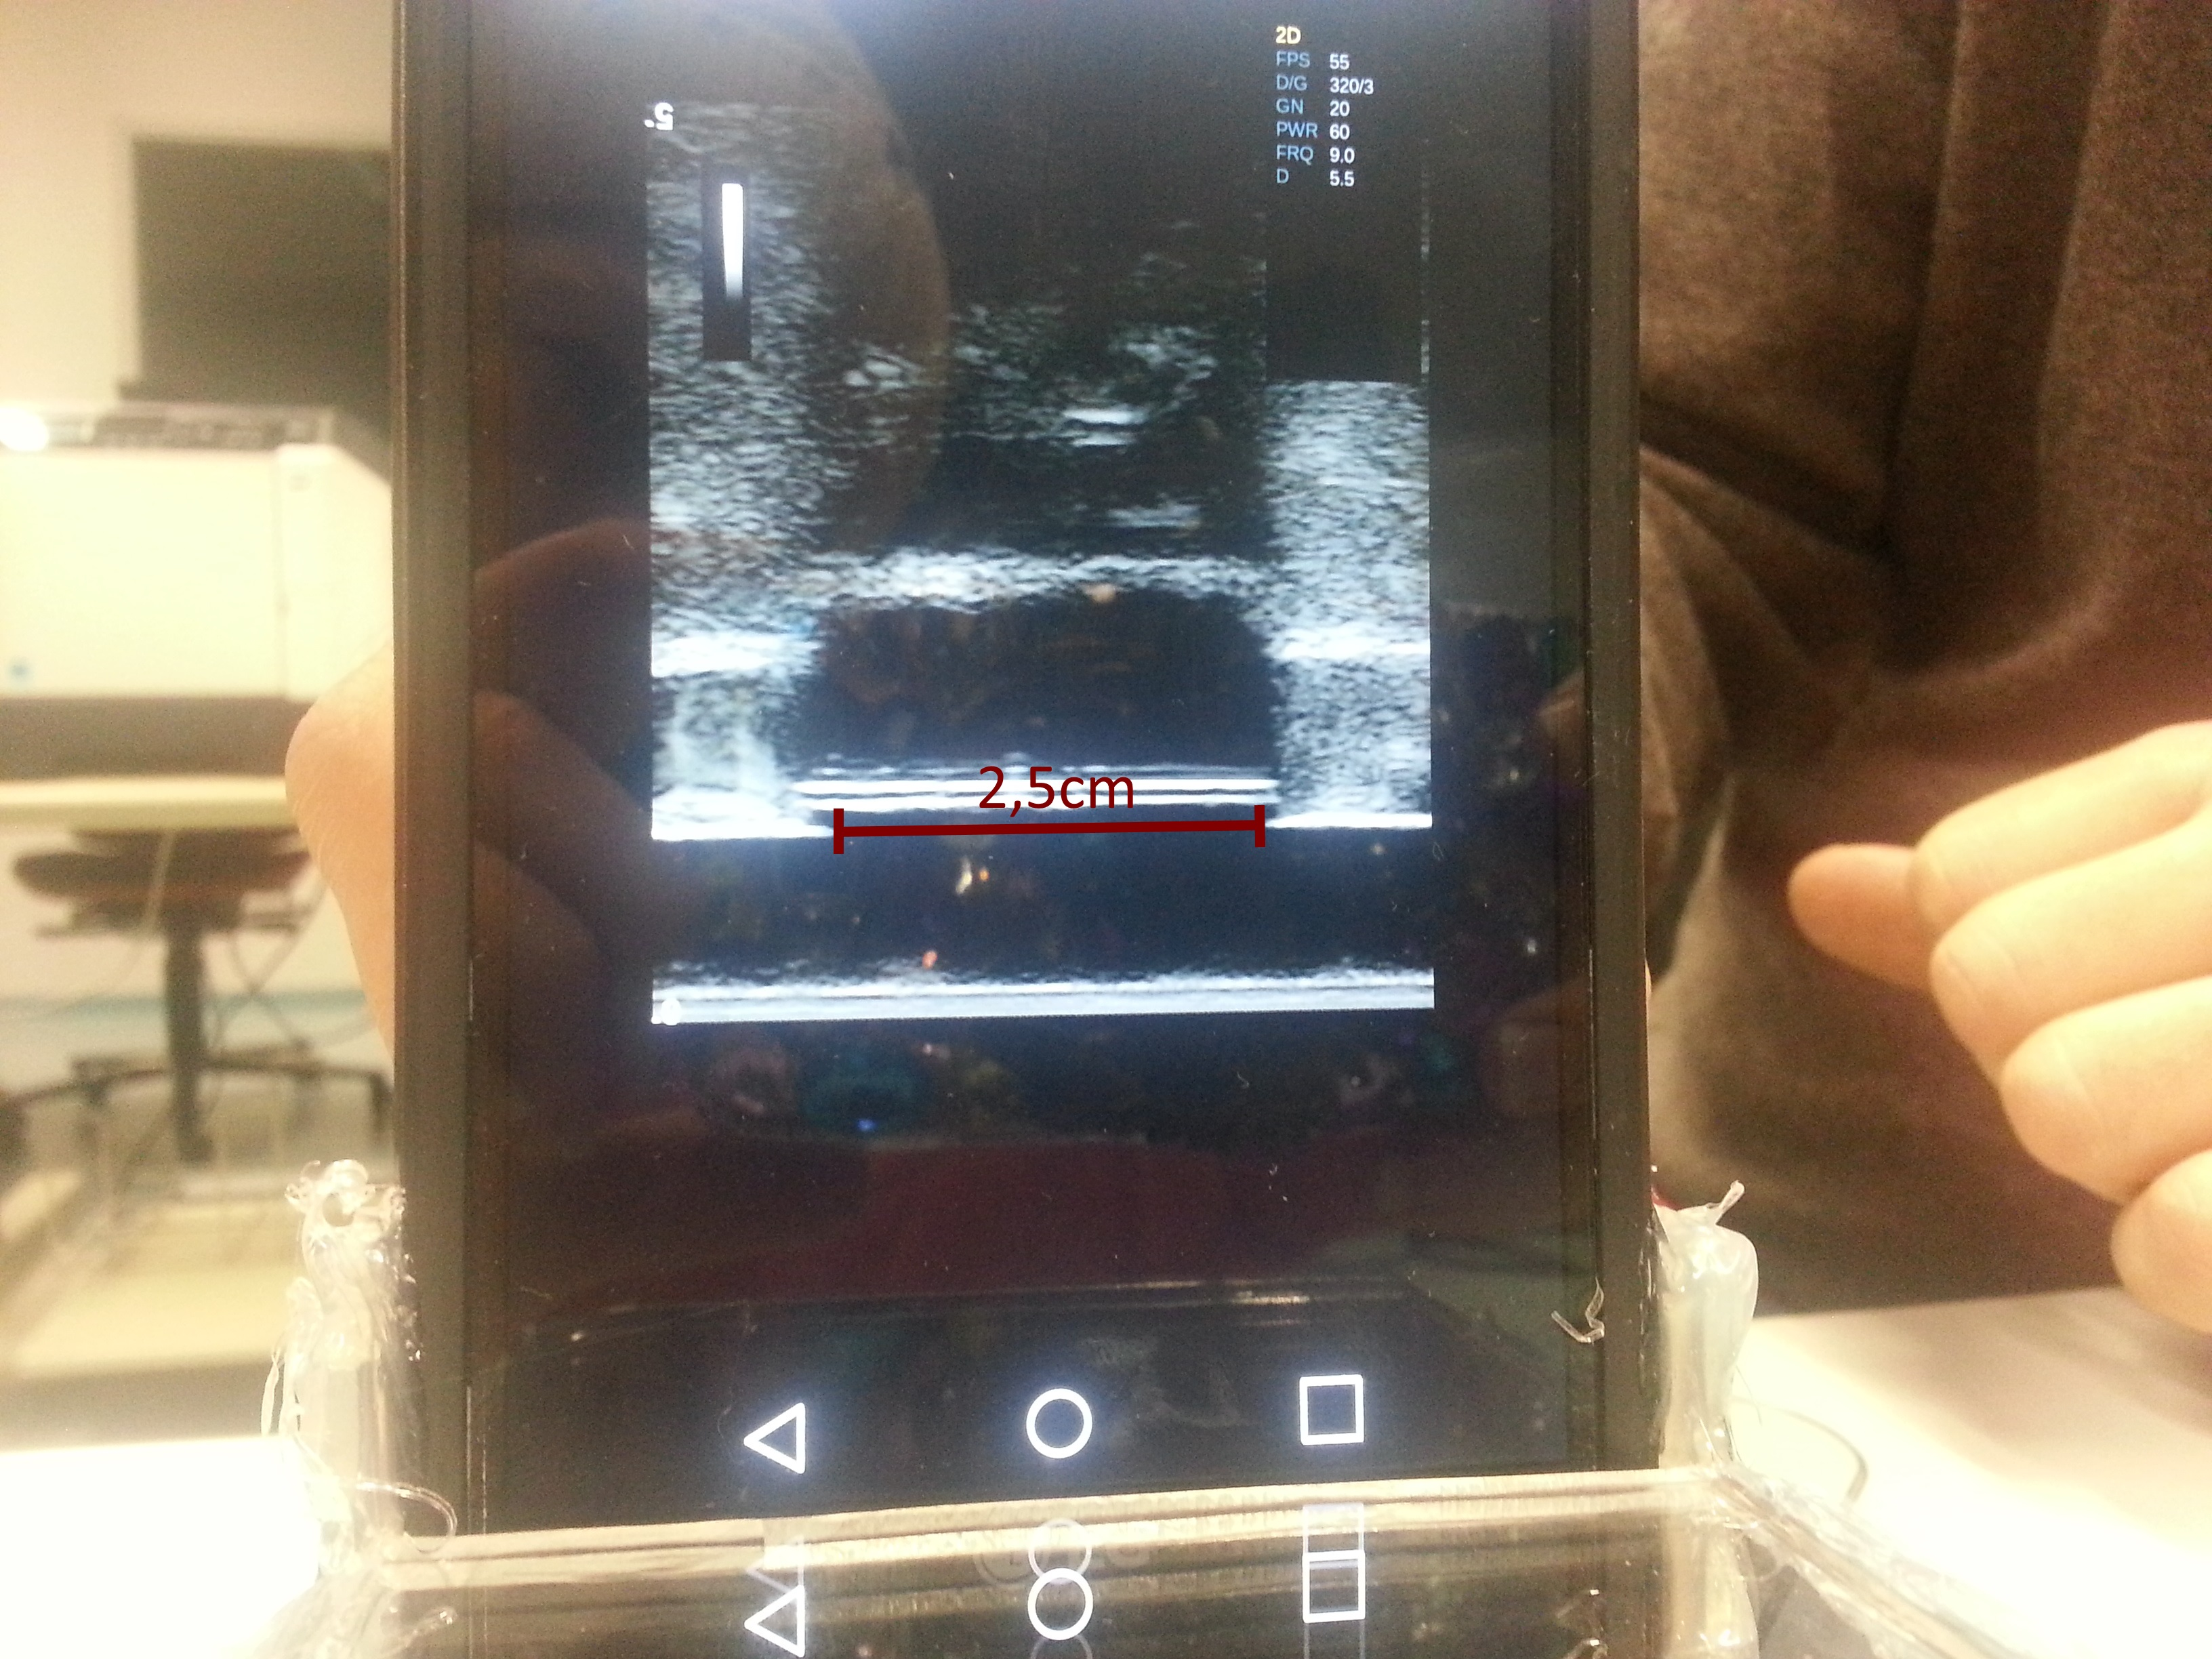
\includegraphics[width=0.7\textwidth]{Bilder/Evaluation/2Muenzen.jpg}
	\caption{Das Schallen beider Münzen in der Gelatineplatte}
	\label{fig:2Muenzen}
\end{figure}

~\\
Abschließend sind nachfolgend noch einmal alle Messergebnisse tabellarisch aufgelistet.
\\
\\
\begin{tabular}{lll}
\textbf{Objekt} & \textbf{Reales Maß in cm} & \textbf{Projiziertes Maß in cm}\\
Tiefe zur Münze & 1,3 & 1,3\\
1 Cent Münze & 1,625 & 1,8\\
Abstand zwischen den Münzen & 2,5 & 2,5\\
\end{tabular}

